\section{Transferencia a artistas principales no vistos}

Como diagnóstico secundario se definió el grupo por el primer nombre de
\code{artists} antes de \code{;}, sin espacios laterales y sin distinguir
mayúsculas. \code{GroupShuffleSplit} con semilla 42 reservó 18.193 canciones de
3.528 artistas principales para prueba y 71.547 canciones de 14.111 artistas
principales para entrenamiento. Dentro de este último se separaron 57.176 para
ajuste y 14.371 para validación agrupada. La selección de parámetros se repitió
allí desde cero, sin usar la validación aleatoria. La huella SHA-256 de los IDs
de prueba agrupada es:

{\footnotesize\ttfamily\noindent a76b54b8e2fd914db9dc5984ff77a8ac07e5b13bf0f36b7e371d048194e5ac52\par}

No hay artistas \emph{principales} compartidos entre entrenamiento y prueba. Sí
hay 1.732 nombres que figuran como artistas secundarios en canciones de prueba y
aparecen en entrenamiento en algún rol; 2.633 canciones de prueba contienen al
menos uno. Este diagnóstico no equivale a una prueba con todos los colaboradores
nuevos. El 20\,\% de \code{GroupShuffleSplit} se refiere a grupos, por lo que no
exige un 20\,\% exacto de canciones.

\begin{table}[htbp]
\centering\small
\begin{tabular}{llrrrr}
\toprule
Predictores & Modelo & MAE & RMSE & $R^2$ & Mejora MAE \\
\midrule
Referencia & Mediana & 16,707 & 20,075 & $-0,003$ & 0,000 \\
Completo & Ridge & 12,102 & 16,740 & 0,302 & 4,605 \\
Completo & Árbol & 14,455 & 18,247 & 0,171 & 2,252 \\
Sin géneros & Ridge & 16,245 & 19,855 & 0,019 & 0,462 \\
Sin géneros & Árbol & 15,703 & 19,652 & 0,039 & 1,004 \\
Solo géneros & Ridge & 12,120 & 16,763 & 0,301 & 4,587 \\
Solo géneros & Árbol & 14,500 & 18,268 & 0,169 & 2,207 \\
\bottomrule
\end{tabular}
\caption{Prueba por artista principal, $n=18.193$. Cada variante eligió parámetros dentro de la partición agrupada.}
\label{tab:artist-test}
\end{table}

Ridge completo mantuvo una mejora frente a su referencia (27,6\,\% en MAE,
frente a 30,9\,\% en la partición aleatoria). Los MAE 12,102 y 11,915 no
corresponden a las mismas canciones; su diferencia no mide por sí sola el efecto
causal de excluir artistas ya vistos. La popularidad es histórica y la muestra
conserva el sesgo por género.

\section{Errores extremos y ranking retrospectivo}

El MAE global de Ridge completo oculta extremos difíciles. En las 653 canciones
con popularidad real al menos 70, el MAE fue 36,759 y la mediana predicha 40,035;
todas recibieron una predicción menor que 70. En las 1.863 canciones de
popularidad cero, el MAE fue 24,448 y la mediana predicha 23,369. Hubo 651
errores absolutos de al menos 40 puntos: 236 fueron canciones de popularidad al
menos 70 y 278 tuvieron popularidad cero. El rango predicho fue aproximadamente
$-31,636$ a 79,706; 76 predicciones quedaron bajo cero porque Ridge no restringe
su salida a 0--100. Se conservaron esos valores para el diagnóstico, sin ajustar
una corrección al mirar la prueba.

\begin{figure}[htbp]
\centering
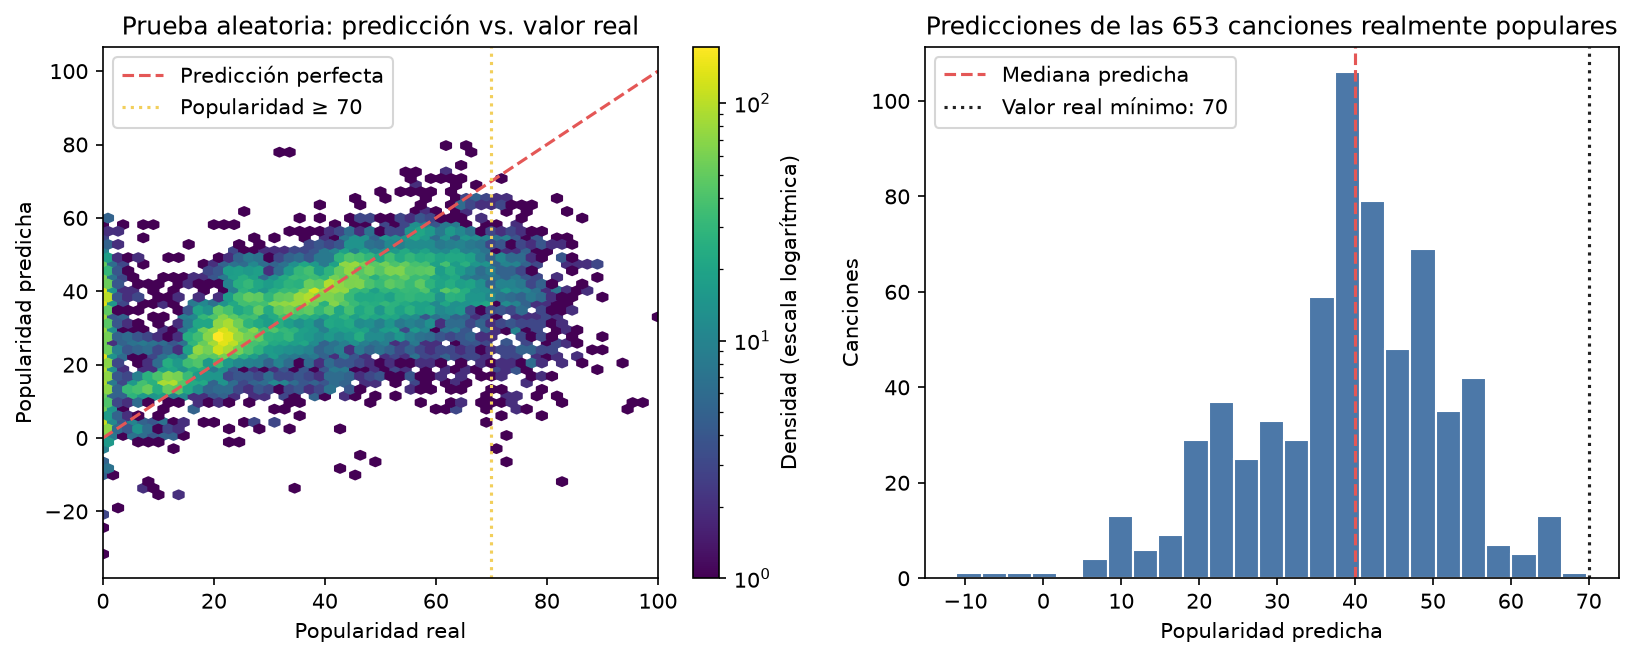
\includegraphics[width=\linewidth]{04a_lucas_predictions_vs_actual.png}
\caption{Valor predicho frente al real y distribución de predicciones de las 653 canciones realmente populares. La concentración intermedia explica subestimaciones grandes en el extremo alto.}
\label{fig:predictions}
\end{figure}

El modelo no contiene identidad de artista, fecha ni exposición promocional.
Esa ausencia es una explicación plausible de su dificultad para distinguir un
éxito excepcional o un cero entre canciones de géneros y perfiles parecidos,
pero los datos no permiten asignar una causa individual a cada error. El MAE
fue 14,198 en canciones \code{explicit=True} ($n=1.517$) y 11,704 en
\code{explicit=False} ($n=16.431$); los soportes son distintos y la diferencia
no demuestra un efecto de la explicitud.

El KPI utiliza una capacidad prefijada de 1.795 canciones (10\,\% redondeado
hacia arriba), popularidad real al menos 70 y desempate por \code{track_id}.
Precisión es la proporción de populares dentro de la lista; recall es la
proporción recuperada de las 653 populares de la prueba; lift divide la precisión
por la prevalencia de 3,64\,\% en \emph{esta muestra}.

\begin{table}[htbp]
\centering\small
\begin{tabular}{lrrrr}
\toprule
Ranking del 10\,\% & Populares halladas & Precisión & Recall & Lift \\
\midrule
Referencia mediana & 63 & 3,5\,\% & 9,6\,\% & 0,965 \\
Ridge completo & 159 & 8,9\,\% & 24,3\,\% & 2,435 \\
Ridge sin géneros & 136 & 7,6\,\% & 20,8\,\% & 2,082 \\
Árbol completo & 119 & 6,6\,\% & 18,2\,\% & 1,822 \\
Árbol sin géneros & 82 & 4,6\,\% & 12,6\,\% & 1,256 \\
\bottomrule
\end{tabular}
\caption{Ranking retrospectivo de las variantes declaradas. Porcentajes redondeados.}
\label{tab:kpi}
\end{table}

Al incluir géneros, Ridge recupera 23 populares adicionales respecto a la
variante sin géneros, y el árbol 37. El ranking de Ridge completo supera una
selección aleatoria de igual tamaño en esta muestra, pero deja fuera 494 de las
653 populares y selecciona 1.636 que no alcanzan el umbral. El lift no acredita
utilidad comercial: la fuente ya contiene popularidad histórica y el modelo
falla en los extremos absolutos.
